\documentclass[aspectratio=169]{beamer}

% 16:9 has textwidth 398.3386pt
% 4:3 has textwidth 307.28987pt.

\usetheme[numbering=none, progressbar=frametitle]{metropolis}
\usepackage[lf]{FiraSans}
\usepackage{bm}
\usepackage{booktabs}
\usepackage{siunitx}
\usepackage{tikz}
\bibliographystyle{plainnat}
\graphicspath{{fig/}}

\pagenumbering{gobble}


\author{Jack Walton}
\title{Bayesian Statistics in Astrophysics}
\institute{Newcastle University}
\date{November 26, 2019}

\begin{document}

\begin{frame}
  \tikz [remember picture,overlay]
  \node at
    ([yshift=2.5cm,xshift=5.42cm]current page.south) 
    {
\includegraphics[width=.25\textwidth,height=.25\textwidth]{qr.png}};
  \titlepage
\end{frame}


\begin{frame}{This talk's not \emph{really} about astrophysics\ldots}
  \begin{columns}
    \begin{column}{0.6\textwidth}
      The second part of this talk makes a case study using astrophysical data\\\vspace{0.5cm}
      However, the methodolgy we'll explore can be used to model \emph{any} observation
      which varies through time. 
    \end{column}%
    \begin{column}{0.4\textwidth}
      \vspace{-0.75cm}
      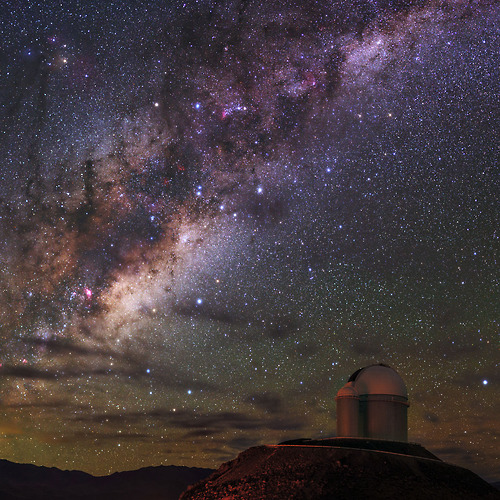
\includegraphics[width=0.9\textwidth, height=\textwidth]{space.jpg}
    \end{column}
  \end{columns}
\end{frame}

\begin{frame}{A tale of two parts}
  \begin{itemize}
    \item Bayesian \&  frequentist statistics
    \begin{itemize}
      \item The two approaches and how they differ
      \item An introduction to MCMC and Stan
    \end{itemize}
  \end{itemize}
  \begin{itemize}
    \item Sunspot occurrence
    \begin{itemize}
      \item What they are and why we should care
      \item Autoregressive models
      \item Model fitting and results
    \end{itemize}
  \end{itemize}
\end{frame}

\section{Bayesian \& frequentist statistics}

\begin{frame}{Frequentist statistics}
  \begin{columns}
    \begin{column}{0.6\textwidth}
      \begin{itemize}
        \item This approach to statistics will be familiar to most
        \item \emph{Think} $p$-values, hypothesis testing, confidence intervals etc.
        \item However, it is not the only statistical framework (nor is it the
               focus of this talk\ldots)
      \end{itemize}
    \end{column}%
    \begin{column}{0.4\textwidth}
      \centering
      \vspace{-0.75cm}
      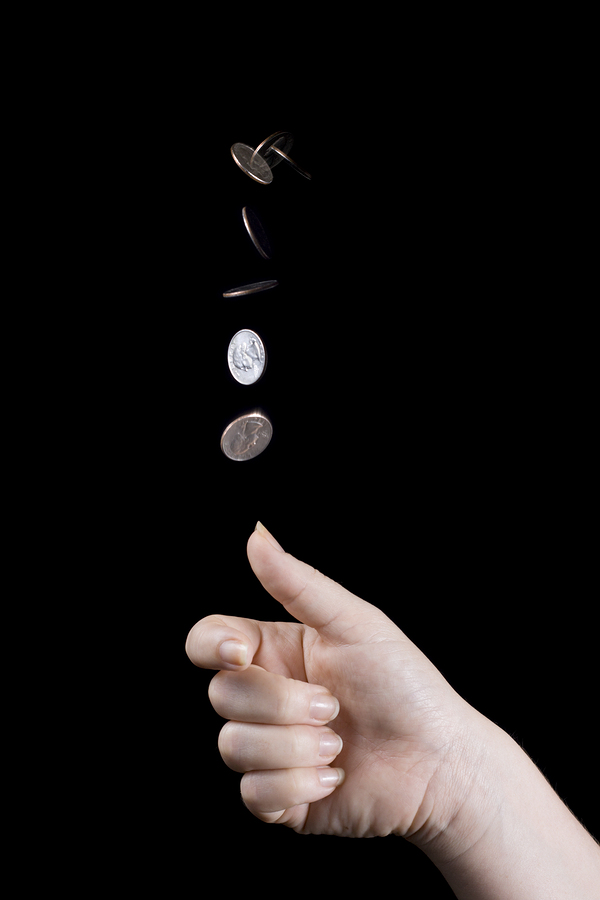
\includegraphics[width=0.75\textwidth]{tosser.jpg}
    \end{column}
  \end{columns}
\end{frame}

\begin{frame}{Bayesian vs. frequentist statistics}
  The difference between Bayesians and frequentists lies in the interpretation
  of probability\ldots

  For a \emph{frequentist}:\\\vspace{0.25cm}
  \begin{quote}
    {\normalfont An event's probability is the limit of its \alert{relative
        frequency in many trials}}
  \end{quote}

  For a \emph{Bayesian}:\\\vspace{0.25cm}
  \begin{quote}
    {\normalfont An event's probability is a \alert{degree of belief}}
  \end{quote}
\end{frame}

\begin{frame}{\emph{Why} Bayesian?}
  \begin{itemize}
    \item Philosophically aligns with how we practice science: \alert{updating}
          our \alert{beliefs} in light of \alert{new evidence}
    \item Allows the inclusion of expert information through a \alert{prior
            distribution}
    \item For events that only occur once, how appropriate is a methodology
          which relies on repeatability?
  \end{itemize}
\end{frame}

\begin{frame}{Bayes' Theorem}
  \begin{columns}
    \begin{column}{0.6\textwidth}
      \vspace{1em}
      \begin{equation*}
        \pi(\theta \,|\,\bm{x}) = \frac{\pi(\theta)\,L(\bm{x}\,|\,\theta)}{\int_{\Theta} \pi(\bm{x}\,|\,\theta)\, \text{d}\theta}
      \end{equation*}
      \begin{itemize}
        \setlength\itemsep{1em}
        \item $\pi(\theta)$ represents our \alert{prior} beliefs
        \item $L(\bm{x}\,|\,\theta)$ is the likelihood of observing $\bm{x}$ given the model \& parameters $\theta$
        \item $\int_{\Theta} \pi(\bm{x}\,|\,\theta)\, \text{d}\theta$ is the normalising constant (probability of $\bm{x})$
        \item $\pi(\theta \, | \, \bm{x})$ represents our \alert{posterior} beliefs
      \end{itemize}
    \end{column}
    \begin{column}{0.4\textwidth}
      \begin{figure}
        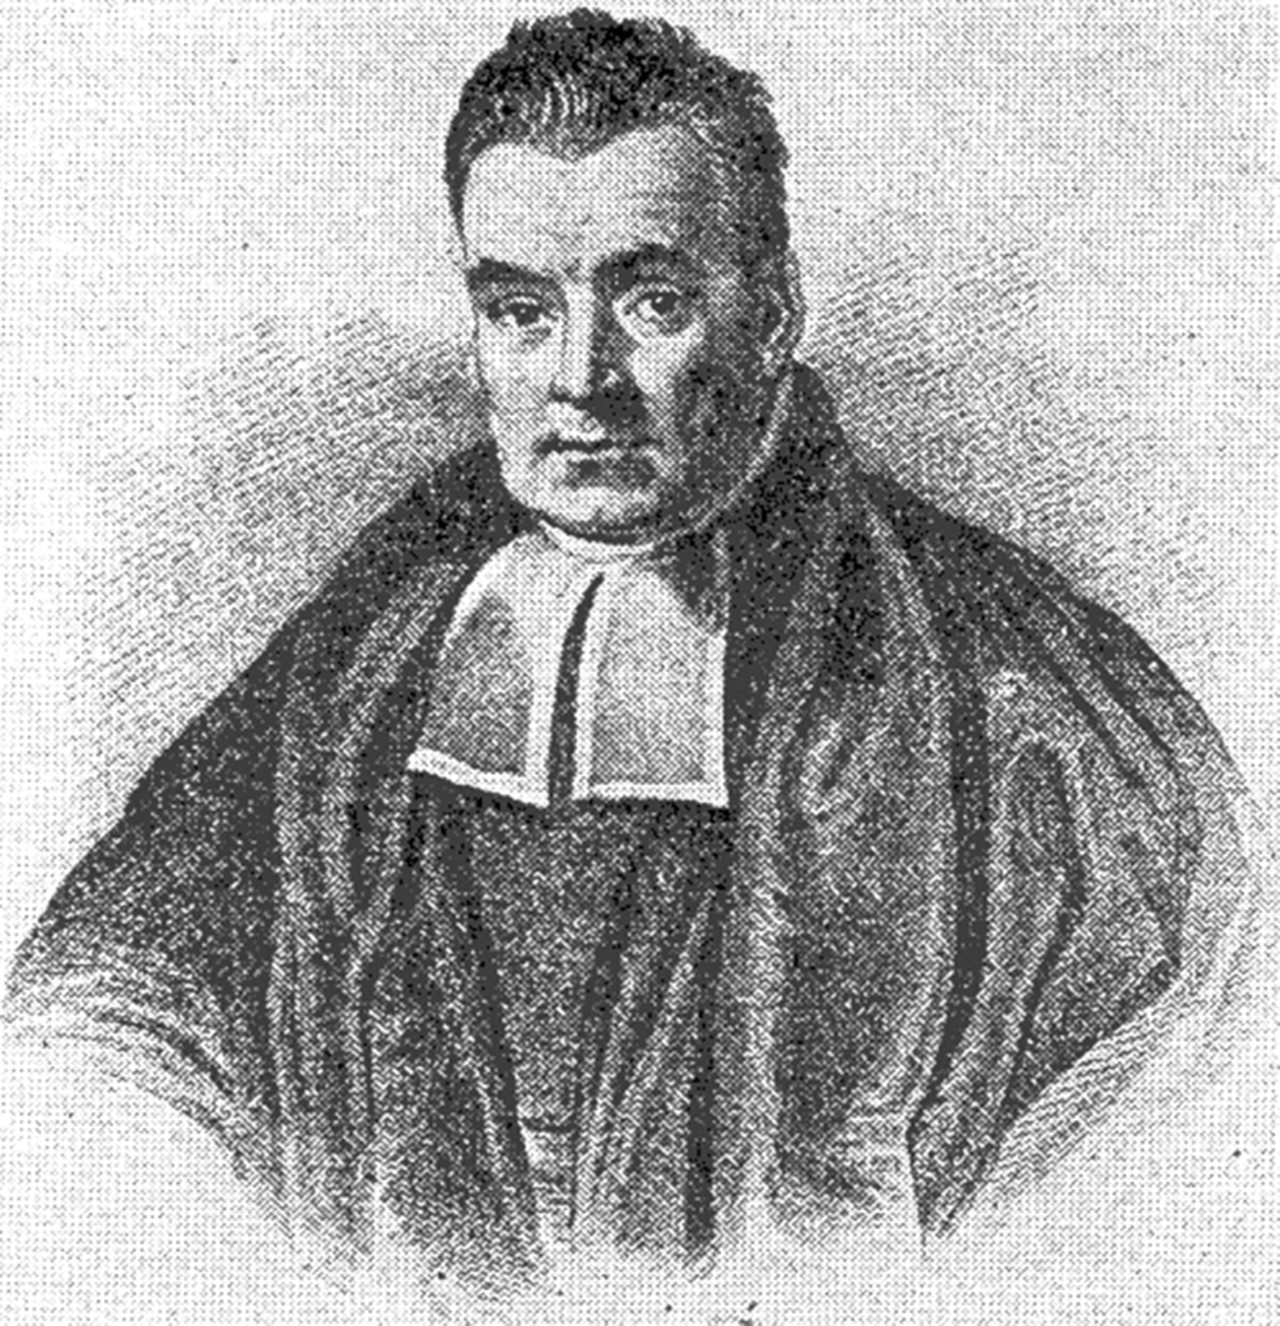
\includegraphics[width=\textwidth]{baes.jpg}
        \caption{Purportedly Bayes}
      \end{figure}
    \end{column}
  \end{columns}
\end{frame}

% naughty
\setcounter{figure}{0}

\begin{frame}{Bayes' Theorem}
  \begin{columns}
    \begin{column}{0.6\textwidth}
      Typically, $\int_{\Theta} \pi(\bm{x}\,|\,\theta)\, \text{d}\theta$ is \emph{very} difficult to compute.\\\vspace{0.5cm}

      Instead we often consider:

      \begin{align*}
        \pi(\theta\,|\,\bm{x}) & \propto \pi(\theta) \times L(\bm{x}\,|\,\theta) \\
        \text{posterior}       & \propto \text{prior} \times \text{likelihood}
      \end{align*}
    \end{column}
    \begin{column}{0.4\textwidth}
      \begin{figure}
        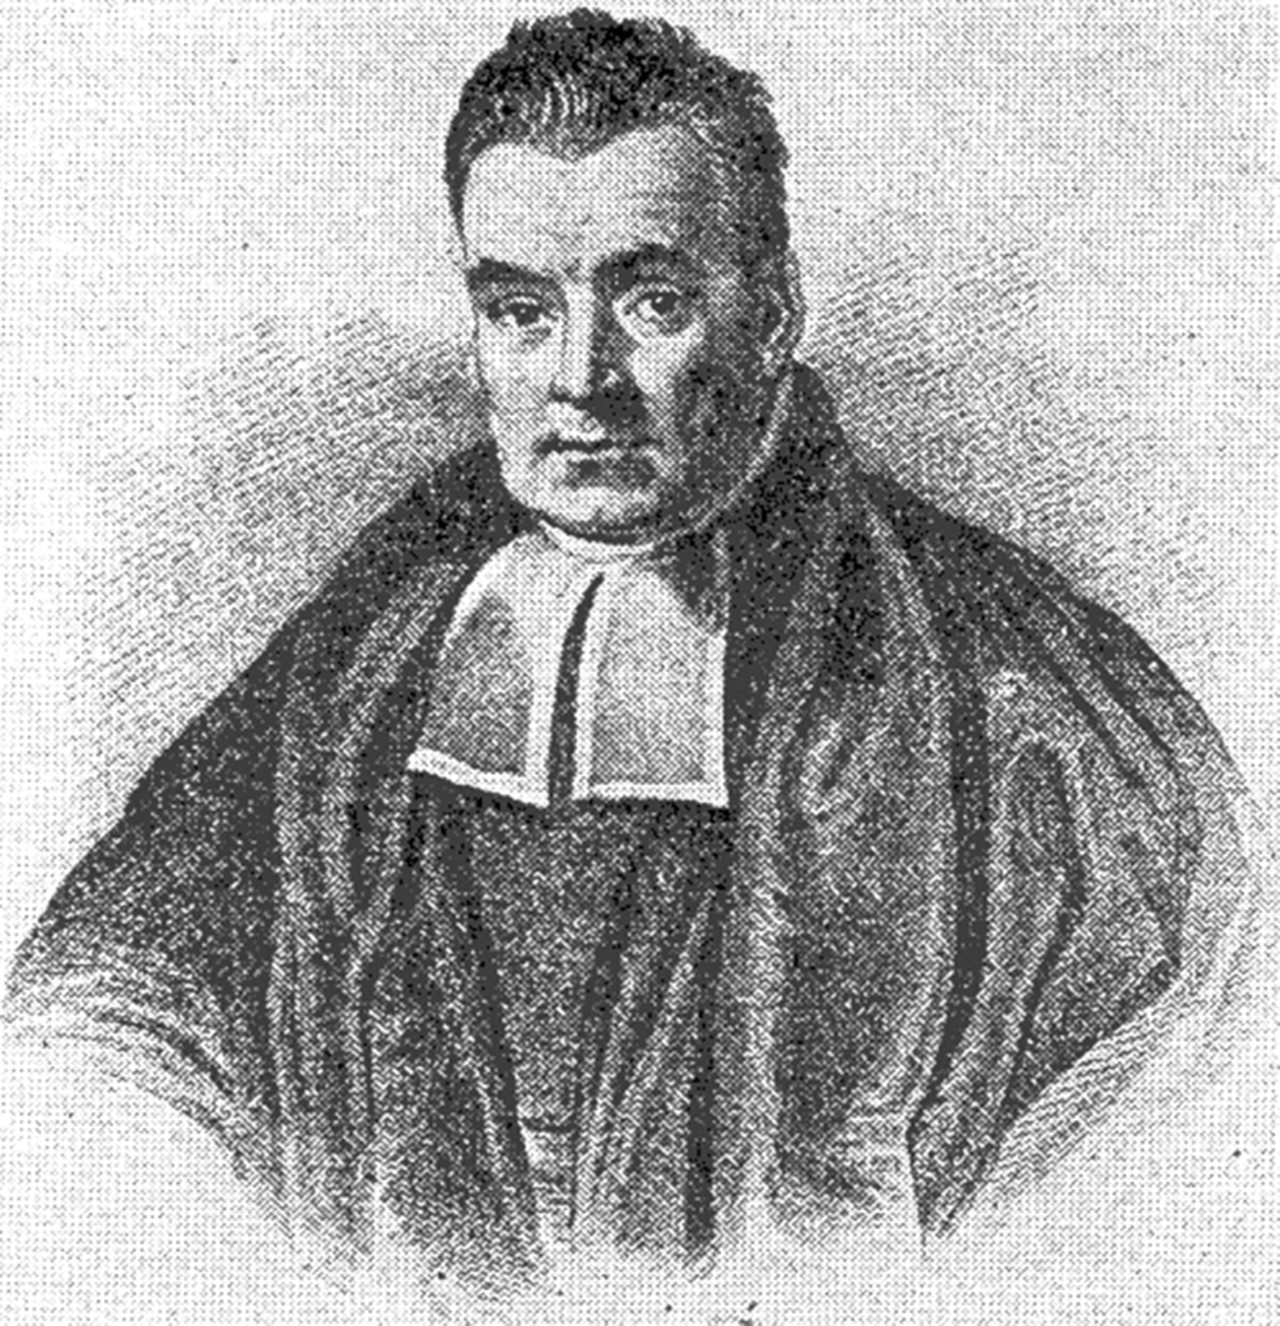
\includegraphics[width=\textwidth]{baes.jpg}
        \caption{Purportedly Bayes}
      \end{figure}
    \end{column}
  \end{columns}
\end{frame}

\begin{frame}{MCMC}
  \begin{columns}
    \begin{column}{0.6\textwidth}
  \begin{itemize}
    \item MCMC --- Markov Chain Monte Carlo
    \item Class of algorithms used to sample from probability densities
    \item We can use them to sample from $\pi(\theta \, | \, \bm{x})$, our
          posterior distribution
    \item Avoids the computation of $\pi(\bm{x})$
  \end{itemize}
  \end{column}%
  \begin{column}{0.4\textwidth}
    \centering
    \vspace{-0.6cm}
    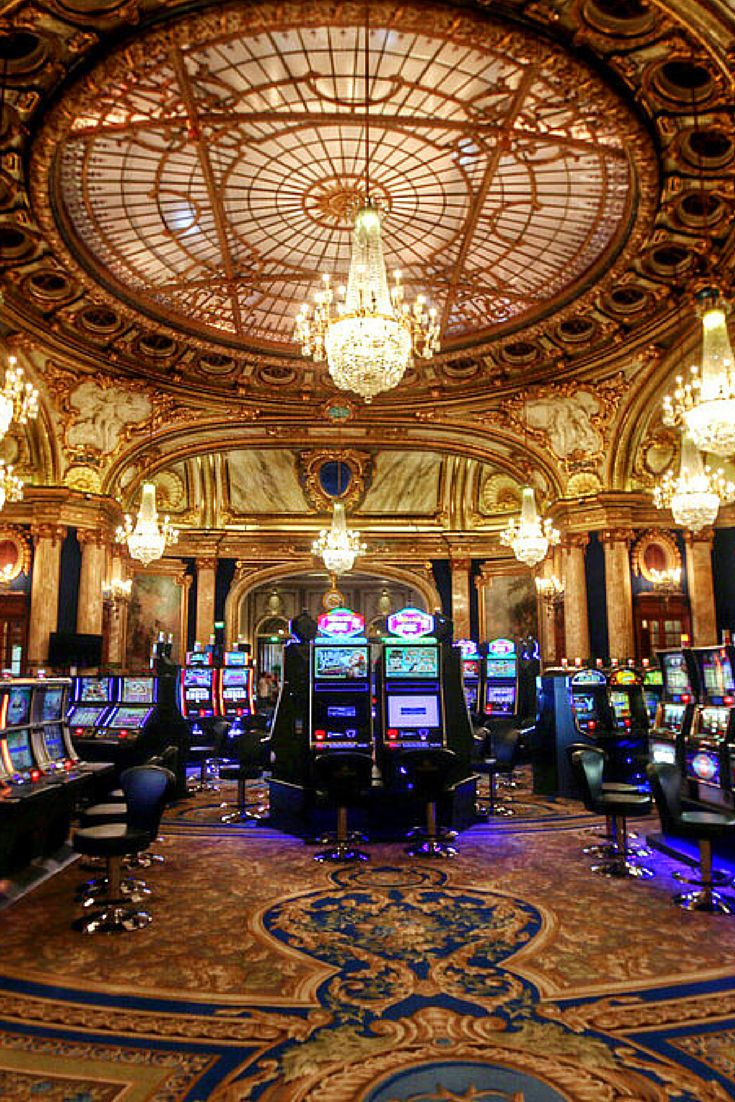
\includegraphics[width=0.8\textwidth]{mc.jpg}
  \end{column}
  \end{columns}
\end{frame}

\begin{frame}{Stan}
  \begin{columns}
    \begin{column}{0.6\textwidth}
      \begin{itemize}
        \item Probabilistic programming language wrote in C++. Accessed via
              interfaces with Python, R, Matlab, Julia\ldots
        \item Stan implements current state-of-the-art MCMC algorithms
        \item Named after Stanislaw Ulam, a mathematician and nuclear physicist and
              pioneer of Monte-Carlo methods.
      \end{itemize}
    \end{column}
    \begin{column}{0.4\textwidth}
      \begin{figure}
        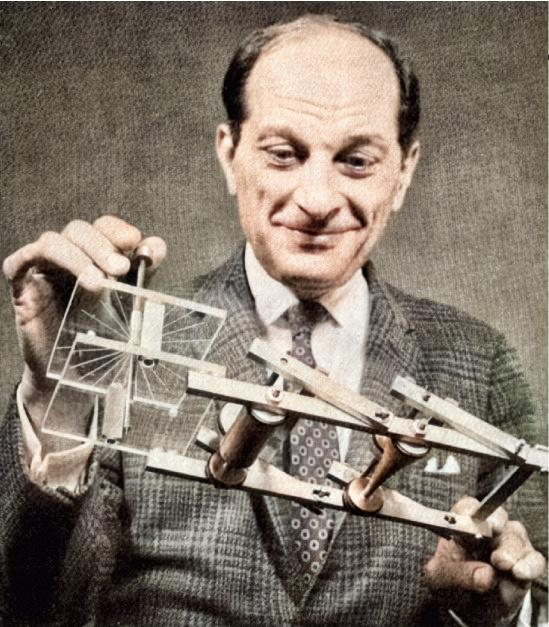
\includegraphics[width=0.9\textwidth]{stan.jpg}
        \caption{Stanislaw \& the FERMIAC}
      \end{figure}
    \end{column}
  \end{columns}
\end{frame}

\section{Sunspot occurrence: a case study}

\begin{frame}{What \emph{are} sunspots and who cares anyway?}
  \begin{columns}
    \begin{column}{0.6\textwidth}
      \begin{itemize}
        \item Dark regions which appear on the surface of the sun
        \item Cooler areas, caused by concentrations of magnetic field flux
        \item Precursor to more dramatic events such as solar flares and
              coronal mass ejections
        \item Significant concern for astronauts living in space, airline
              passengers on polar routes and satellite engineers
      \end{itemize}
    \end{column}%
    \begin{column}{0.4\textwidth}
      \begin{figure}
        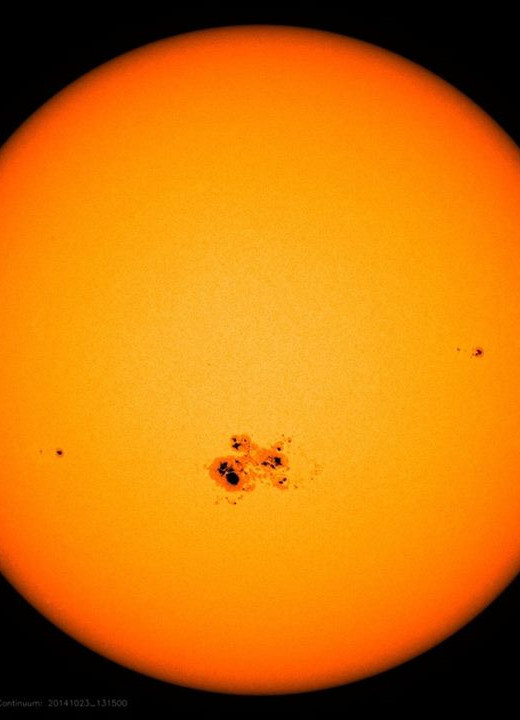
\includegraphics[width=0.8\textwidth]{sun.jpg}
        \caption{Sunspots}
      \end{figure}
    \end{column}
  \end{columns}
\end{frame}

\begin{frame}{The data}
  \begin{columns}
    \begin{column}{0.5\textwidth}
      We shall use the annual data for the International Sunspot number,
      under the responsibility of the Royal Observatory in Belgium since 1980.
    \end{column}
    \begin{column}{0.5\textwidth}
      \vspace{1em}
      \begin{figure}
        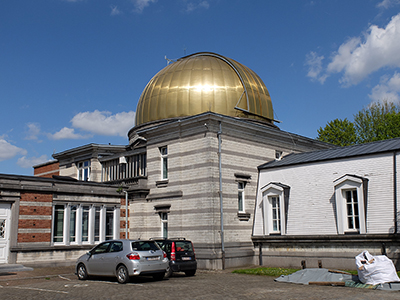
\includegraphics[width=\textwidth]{belgium.JPG}
        \caption{Royal observatory of Belgium}
      \end{figure}
    \end{column}
  \end{columns}
\end{frame}

\begin{frame}{The data}
  \begin{figure}
    \centering
    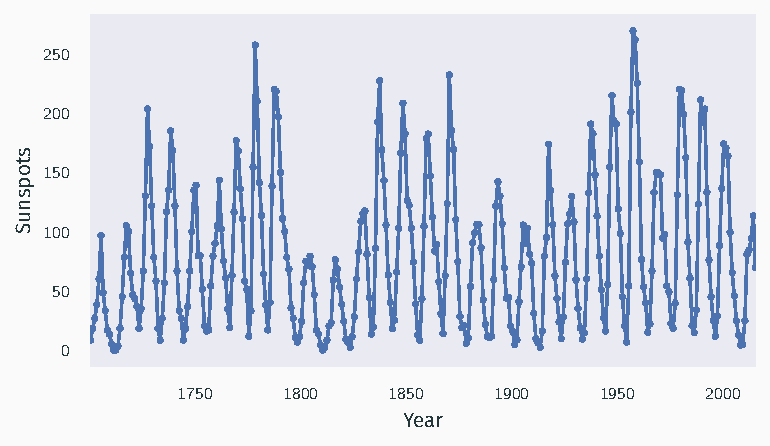
\includegraphics{data.pdf}
  \end{figure}
\end{frame}

\begin{frame}{Autoregressive models}
  Autoregressive models \alert{predict future} behaviour \alert{given past} behaviour

  An $AR(p)$ model:
  \begin{align*}
      & X_{t} \sim Normal(\mu_{t}, \sigma^2) \\
      &  \mu_{t} = \alpha + \varphi_1 X_{t-1} + \varphi_2 X_{t-2} + \varphi_3 X_{t-3} + \ldots +
      \varphi_{t-p} X_{t-p}
  \end{align*}
\end{frame}

\begin{frame}{In the flesh: $AR(1)$ processes}
  \vspace{-0.85cm}
  \begin{figure}
    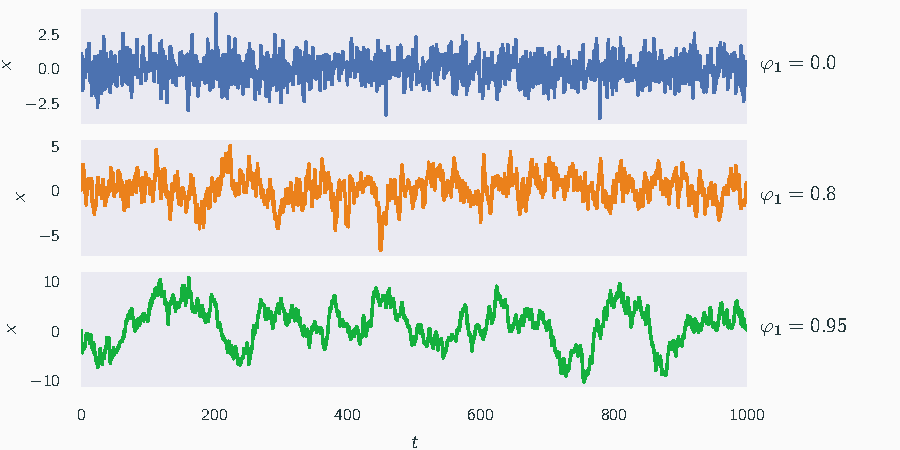
\includegraphics{AR.pdf}
  \end{figure}
\end{frame}

\begin{frame}{Normal $AR(1)$ model}
  \begin{align*}
      S_t \sim Normal(\mu_t, \sigma^2) & \\
      \mu_t = \alpha + \varphi S_{t-1} &
  \end{align*}

  Given the observed data can we infer the parameters $\alpha$,
  $\varphi$ and $\sigma$?
\end{frame}

\begin{frame}{Results: summary}
  \centering
  \begin{table}
    \input{fitting/out/norm.tab}
    \caption{Summary of posterior samples after running Stan for $10\,000$ iterations (3 seconds).}
  \end{table}
\end{frame}

\begin{frame}{Results: posterior densities}
  \begin{figure}
    \centering
    \includegraphics{fitting/out/norm_kde.pdf}
  \end{figure}
\end{frame}

\begin{frame}{Results: posterior predictives}
  \vspace{-0.3cm}
  \begin{figure}
    \centering
    \includegraphics{fitting/out/norm_post_fit.pdf}
  \end{figure}
\end{frame}

\begin{frame}{Negative Binomial $AR(1)$ model}
  \begin{align*}
      S_{t} \sim NB(p_{t}, \theta)            & \\
      p_{t} = \theta / (\theta + \mu_{t})     & \\
      \log(\mu_{t+1}) = \alpha + \varphi S_{t-1} &
  \end{align*}
  Given the observed data can we infer the parameters $\alpha$,
  $\varphi$ and $\theta$?
\end{frame}

\begin{frame}{Results: posterior predictives}
  \vspace{-0.3cm}
  \begin{figure}
    \centering
    \includegraphics{fitting/out/neg_bin_post_fit.pdf}
  \end{figure}
\end{frame}

\begin{frame}{Conclusion}
  \begin{itemize}
    \item Modern computing power is making Bayesian methodologies more accessible
    \item Many `black-box' MCMC implementations make inference (relatively) pain-free
    \item The inclusion of prior information can be useful for 
          events which have limited observational data
  \end{itemize}
\end{frame}

\begin{frame}{\emph{People who liked this also liked\ldots}}
  \centering
  \renewcommand{\arraystretch}{2}
  \setlength\tabcolsep{0.75cm}
  \begin{tabular}{cc}
    Suitable bed time reading:&
    \emph{Not} suitable bed time reading:\\
    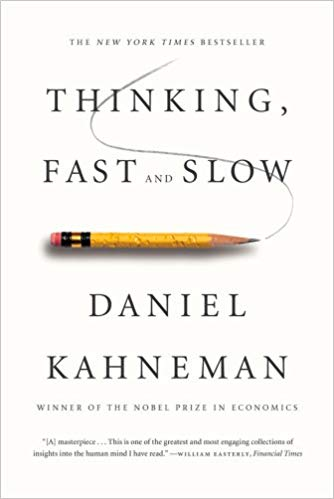
\includegraphics[width=0.275\textwidth]{thinking.jpg}&
    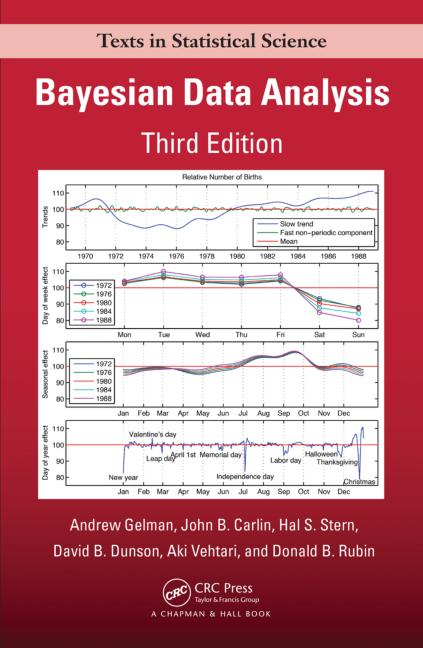
\includegraphics[width=0.275\textwidth]{bda3.jpg} \\
  \end{tabular}
\end{frame}

\begin{frame}{References}
  \nocite{hilbe2017bayesian}
  \bibliography{references.bib}
\end{frame}

\begin{frame}[standout]
  Thanks
\end{frame}

\end{document}
